%%%%%%%%%%%%%%%%%%%%%%%%%%%%%%%%%%%%%%%%%%%%%%%%%%%
% CHƯƠNG 5: XÂY DỰNG MÁY CHỦ TRUNG TÂM VÀ GIAO DIỆN DASHBOARD
%%%%%%%%%%%%%%%%%%%%%%%%%%%%%%%%%%%%%%%%%%%%%%%%%%%
\section*{CHƯƠNG 5. XÂY DỰNG MÁY CHỦ TRUNG TÂM VÀ GIAO DIỆN DASHBOARD}
\addcontentsline{toc}{section}{\numberline{}CHƯƠNG 5. XÂY DỰNG MÁY CHỦ TRUNG TÂM VÀ GIAO DIỆN DASHBOARD}
\setcounter{section}{5}
\setcounter{subsection}{0}
\setcounter{figure}{0}
\setcounter{table}{0}

\subsection{Kiến trúc API Server Node.js và PHP}
Để đảm bảo tính linh hoạt tối đa cho việc tích hợp vào hạ tầng công nghệ thông tin sẵn có của các bệnh viện, hệ thống được phát triển song song hai giải pháp máy chủ API độc lập:
\begin{enumerate}
    \item \textbf{Máy chủ Node.js (\texttt{server.js}):} Được lập trình bằng JavaScript chạy trên môi trường Node.js thuần không phụ thuộc framework bên ngoài. Máy chủ sử dụng mô-đun \texttt{http} tích hợp và cơ chế xử lý không đồng bộ (Asynchronous Event Loop) cho tốc độ tiếp nhận và phản hồi các yêu cầu POST JSON từ hàng trăm thiết bị đeo đồng thời cực kỳ nhanh chóng với độ trễ dưới 50ms.
    \item \textbf{Máy chủ PHP (\texttt{api.php}):} Được xây dựng phục vụ triển khai trên các môi trường máy chủ web Apache/Nginx truyền thống (như bộ phần mềm XAMPP, Laragon). Giải pháp này phù hợp với hạ tầng mạng LAN nội bộ và hệ thống máy chủ sẵn có tại các bệnh viện công lập nhờ tính tương thích cao và cấu hình triển khai đơn giản.
\end{enumerate}

\subsection{Thiết kế cấu trúc dữ liệu lưu trữ JSON cục bộ}
Để tối ưu hóa tốc độ truy cập đọc/ghi dữ liệu và đáp ứng tính nhỏ gọn của đề tài nhúng, hệ thống sử dụng tệp tin phẳng JSON cục bộ \texttt{iot\_store.json} để lưu trữ dữ liệu đo sinh hiệu thay cho các hệ quản trị cơ sở dữ liệu cồng kềnh như MySQL hay SQL Server.

Mỗi khi thiết bị đeo gửi gói tin POST JSON chứa các chỉ số đo, máy chủ đọc nội dung tệp tin \texttt{iot\_store.json}, phân tích chuỗi JSON thành cấu trúc đối tượng, cập nhật dữ liệu sinh hiệu mới nhất của thiết bị dựa trên địa chỉ ID duy nhất của vi điều khiển. Để ngăn chặn kích thước tệp tin JSON tăng lên quá lớn gây tràn bộ nhớ RAM của máy chủ khi hoạt động lâu dài, tôi triển khai thuật toán hàng đợi khống chế số điểm đo lịch sử tối đa cho mỗi bệnh nhân là 120 điểm đo gần nhất:
\begin{lstlisting}
// Cat bot du lieu lich su neu vuot qua 120 diem do gan nhat
if (deviceStore[macAddress].history.length > 120) {
  deviceStore[macAddress].history.shift(); // Xoa diem do cu nhat
}
\end{lstlisting}

\subsection{Thiết kế giao diện Dashboard Web giám sát}
Giao diện Dashboard web giám sát sức khỏe được lập trình bằng HTML5, CSS3 và Vanilla JavaScript theo ngôn ngữ thiết kế tối giản hiện đại (Dark Mode). Dashboard tự động gửi các yêu cầu Ajax HTTP GET đến máy chủ API định kỳ mỗi 3 giây một lần (cơ chế Polling) để cập nhật dữ liệu sinh hiệu mới nhất của tất cả các bệnh nhân đang đeo thiết bị mà không cần tải lại toàn bộ trang web.

\begin{figure}[H]
    \centering
    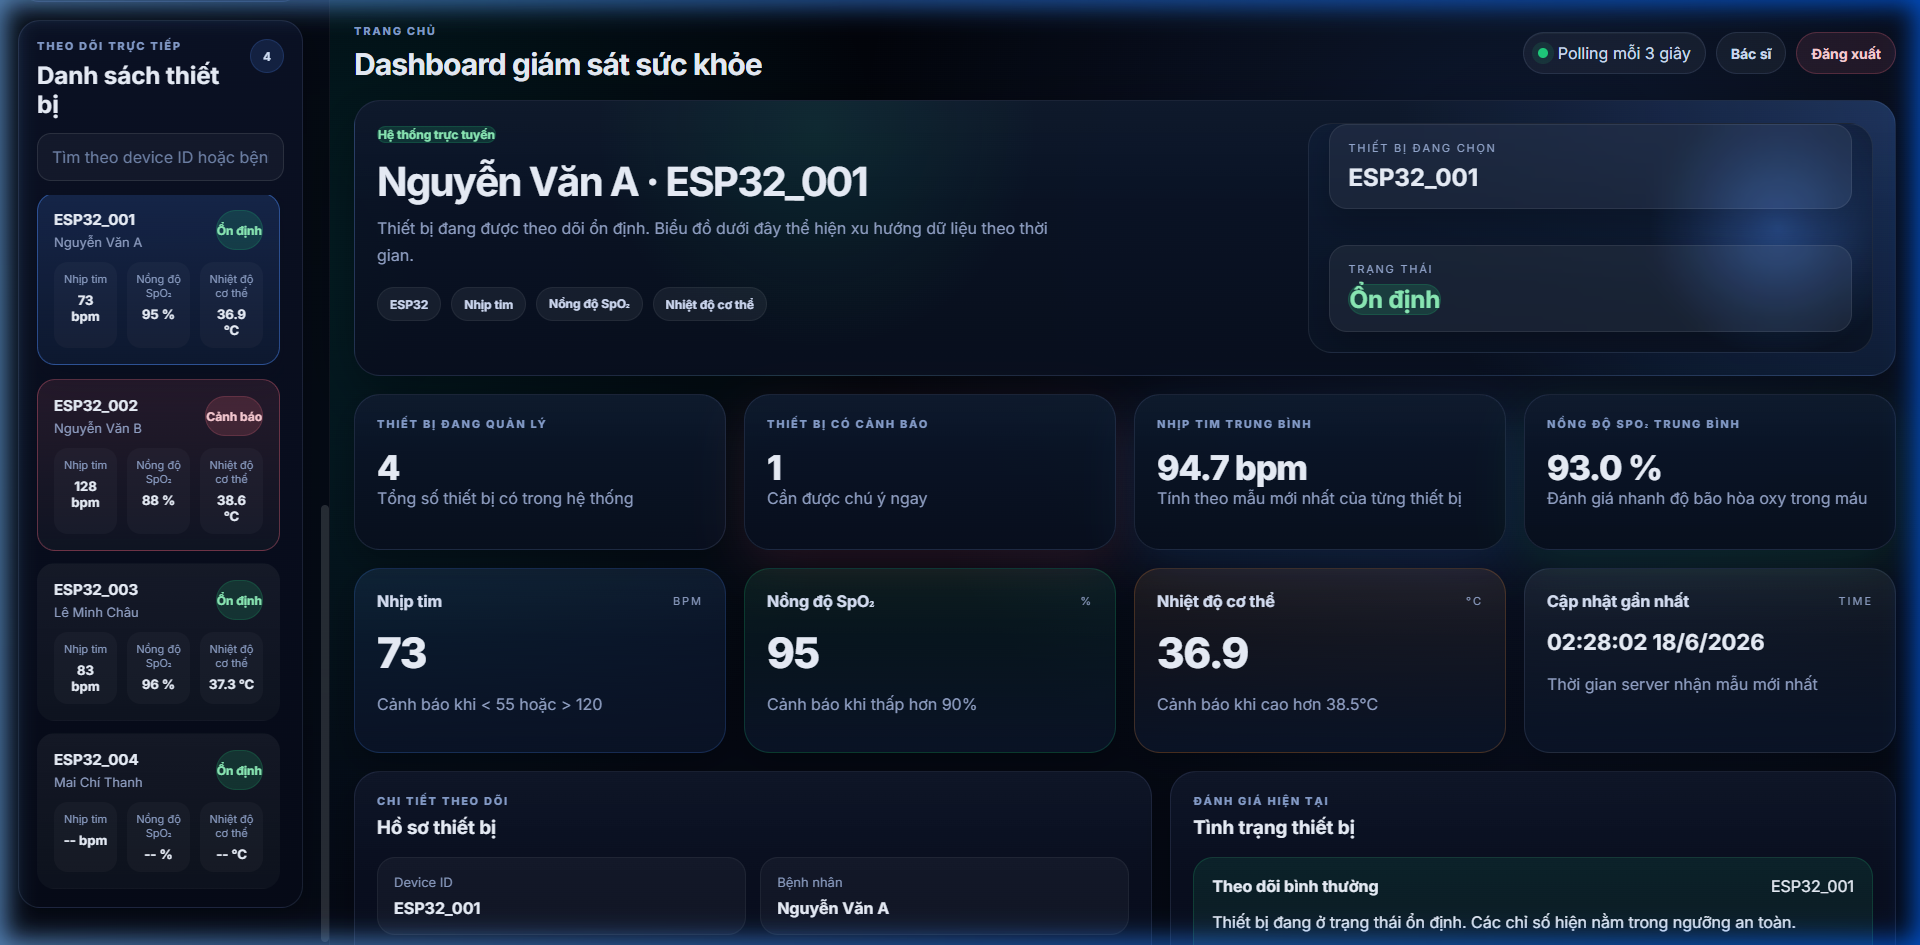
\includegraphics[width=0.95\textwidth]{images/dashboard_overview.png}
    \caption[Giao diện Dashboard Web - Tổng quan chỉ số trực tiếp]{\bfseries\fontsize{12pt}{0pt}\selectfont Giao diện Dashboard Web - Tổng quan chỉ số trực tiếp}
    \label{fig:dashboard_overview}
\end{figure}

\begin{figure}[H]
    \centering
    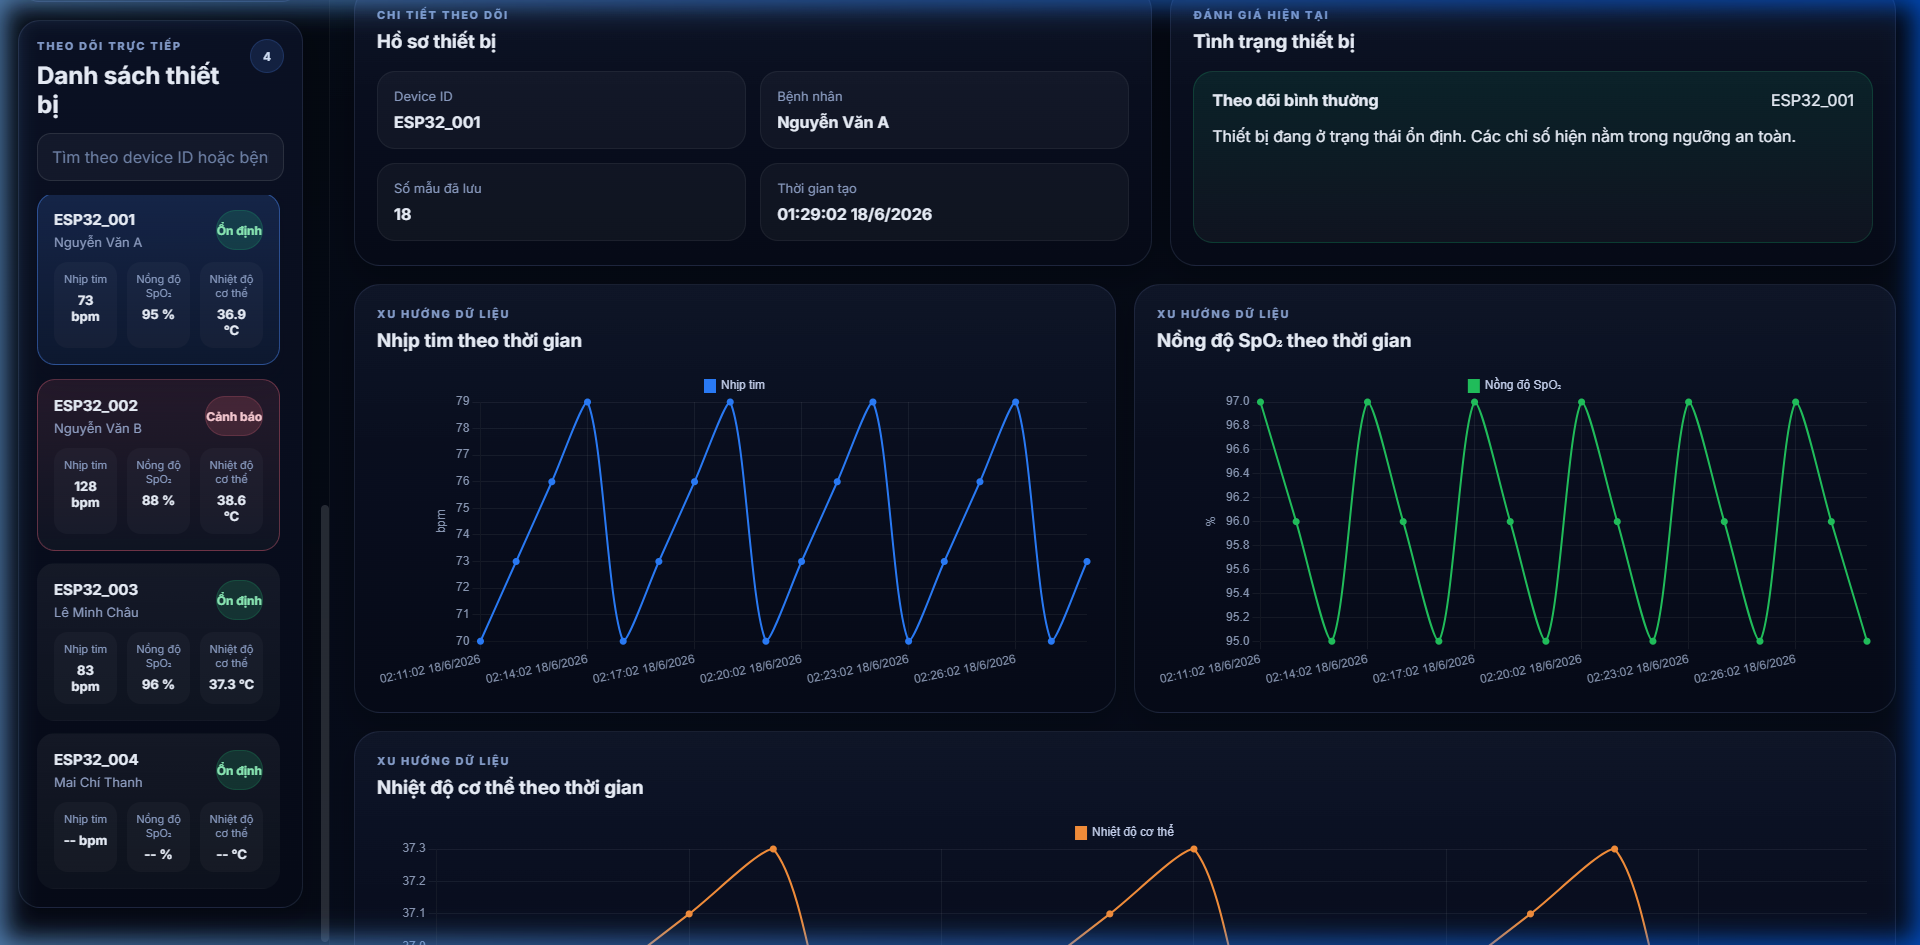
\includegraphics[width=0.95\textwidth]{images/dashboard_charts.png}
    \caption[Giao diện Dashboard Web - Biểu đồ xu hướng sinh hiệu]{\bfseries\fontsize{12pt}{0pt}\selectfont Giao diện Dashboard Web - Biểu đồ xu hướng sinh hiệu}
    \label{fig:dashboard_charts}
\end{figure}

\begin{figure}[H]
    \centering
    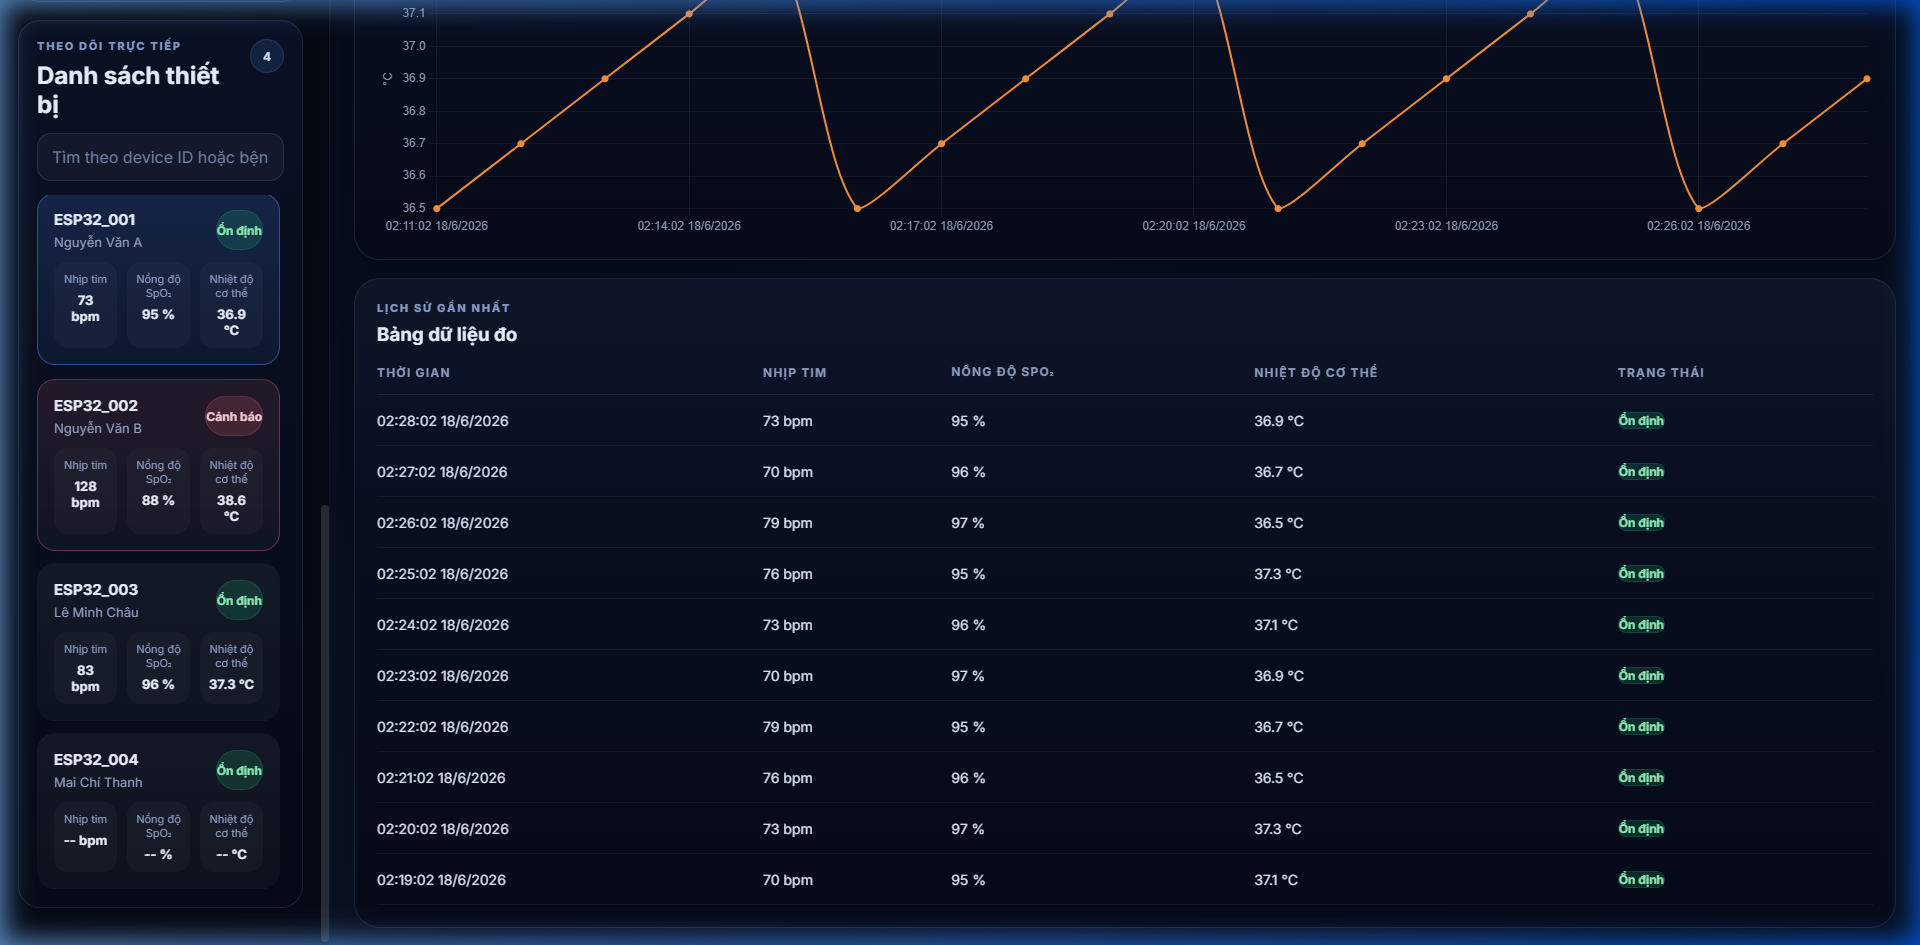
\includegraphics[width=0.95\textwidth]{images/dashboard_history.png}
    \caption[Giao diện Dashboard Web - Bảng lịch sử dữ liệu đo]{\bfseries\fontsize{12pt}{0pt}\selectfont Giao diện Dashboard Web - Bảng lịch sử dữ liệu đo}
    \label{fig:dashboard_history}
\end{figure}

Giao diện hiển thị danh sách các bệnh nhân dưới dạng các thẻ (Card) trực quan. Mỗi chỉ số sinh hiệu (Nhịp tim, $SpO_2$, Thân nhiệt, Độ ẩm) được gán màu sắc cảnh báo động dựa trên các ngưỡng sinh học y tế:
\begin{itemize}
    \item \textbf{Màu xanh lá cây (Trạng thái bình thường):} Nhịp tim $60 - 100\text{ BPM}$, $SpO_2 \ge 95\%$, thân nhiệt $36.5 - 37.4^\circ\text{C}$.
    \item \textbf{Màu vàng/cam (Trạng thái cảnh báo):} Thân nhiệt nhẹ $37.5 - 38.4^\circ\text{C}$ hoặc $SpO_2$ sụt giảm nhẹ $90\% - 94\%$.
    \item \textbf{Màu đỏ nhấp nháy (Trạng thái lâm sàng nguy kịch):} Nhịp tim $< 50\text{ BPM}$ hoặc $> 120\text{ BPM}$, $SpO_2 < 90\%$, hoặc thân nhiệt $> 38.5^\circ\text{C}$ (sốt cao).
\end{itemize}
Khi nhân viên y tế nhấp chọn vào thẻ của một bệnh nhân cụ thể, giao diện sẽ mở rộng hiển thị đồ thị diễn tiến lịch sử trực quan của nhịp tim, $SpO_2$ và thân nhiệt được vẽ bằng thư viện \textbf{Chart.js} (Hình \ref{fig:dashboard_charts}) giúp bác sĩ dễ dàng đánh giá xu hướng tiến triển sức khỏe bệnh nhân và bảng lịch sử dữ liệu đo chi tiết theo thời gian (Hình \ref{fig:dashboard_history}).

\subsection{Cơ chế phân quyền người dùng và bảo mật Session}
Hệ thống tích hợp cơ chế quản lý session dựa trên Cookie trình duyệt để phân quyền hoạt động của nhân viên y tế:
\begin{itemize}
    \item \textbf{Tài khoản Bác sĩ (Doctor -- đăng nhập \texttt{bacsi}):} Có toàn quyền tương tác hệ thống bao gồm xem dữ liệu, cập nhật thông tin cá nhân bệnh nhân, kích hoạt chế độ tạo dữ liệu mẫu ngẫu nhiên (\texttt{seed\_demo}) để chạy kiểm thử và xóa thiết bị khỏi hệ thống.
    \item \textbf{Tài khoản Y tá (Nurse -- đăng nhập \texttt{yta}):} Chỉ có quyền xem danh sách và theo dõi đồ thị trực quan. Mọi yêu cầu can thiệp chỉnh sửa thông tin hoặc xóa thiết bị gửi qua API từ tài khoản y tá đều bị máy chủ từ chối và trả về mã lỗi bảo mật \texttt{403 Forbidden}.
\end{itemize}
